% Options for packages loaded elsewhere
\PassOptionsToPackage{unicode}{hyperref}
\PassOptionsToPackage{hyphens}{url}
\documentclass[
]{article}
\usepackage{xcolor}
\usepackage[margin=1in]{geometry}
\usepackage{amsmath,amssymb}
\setcounter{secnumdepth}{-\maxdimen} % remove section numbering
\usepackage{iftex}
\ifPDFTeX
  \usepackage[T1]{fontenc}
  \usepackage[utf8]{inputenc}
  \usepackage{textcomp} % provide euro and other symbols
\else % if luatex or xetex
  \usepackage{unicode-math} % this also loads fontspec
  \defaultfontfeatures{Scale=MatchLowercase}
  \defaultfontfeatures[\rmfamily]{Ligatures=TeX,Scale=1}
\fi
\usepackage{lmodern}
\ifPDFTeX\else
  % xetex/luatex font selection
\fi
% Use upquote if available, for straight quotes in verbatim environments
\IfFileExists{upquote.sty}{\usepackage{upquote}}{}
\IfFileExists{microtype.sty}{% use microtype if available
  \usepackage[]{microtype}
  \UseMicrotypeSet[protrusion]{basicmath} % disable protrusion for tt fonts
}{}
\makeatletter
\@ifundefined{KOMAClassName}{% if non-KOMA class
  \IfFileExists{parskip.sty}{%
    \usepackage{parskip}
  }{% else
    \setlength{\parindent}{0pt}
    \setlength{\parskip}{6pt plus 2pt minus 1pt}}
}{% if KOMA class
  \KOMAoptions{parskip=half}}
\makeatother
\usepackage{color}
\usepackage{fancyvrb}
\newcommand{\VerbBar}{|}
\newcommand{\VERB}{\Verb[commandchars=\\\{\}]}
\DefineVerbatimEnvironment{Highlighting}{Verbatim}{commandchars=\\\{\}}
% Add ',fontsize=\small' for more characters per line
\usepackage{framed}
\definecolor{shadecolor}{RGB}{248,248,248}
\newenvironment{Shaded}{\begin{snugshade}}{\end{snugshade}}
\newcommand{\AlertTok}[1]{\textcolor[rgb]{0.94,0.16,0.16}{#1}}
\newcommand{\AnnotationTok}[1]{\textcolor[rgb]{0.56,0.35,0.01}{\textbf{\textit{#1}}}}
\newcommand{\AttributeTok}[1]{\textcolor[rgb]{0.13,0.29,0.53}{#1}}
\newcommand{\BaseNTok}[1]{\textcolor[rgb]{0.00,0.00,0.81}{#1}}
\newcommand{\BuiltInTok}[1]{#1}
\newcommand{\CharTok}[1]{\textcolor[rgb]{0.31,0.60,0.02}{#1}}
\newcommand{\CommentTok}[1]{\textcolor[rgb]{0.56,0.35,0.01}{\textit{#1}}}
\newcommand{\CommentVarTok}[1]{\textcolor[rgb]{0.56,0.35,0.01}{\textbf{\textit{#1}}}}
\newcommand{\ConstantTok}[1]{\textcolor[rgb]{0.56,0.35,0.01}{#1}}
\newcommand{\ControlFlowTok}[1]{\textcolor[rgb]{0.13,0.29,0.53}{\textbf{#1}}}
\newcommand{\DataTypeTok}[1]{\textcolor[rgb]{0.13,0.29,0.53}{#1}}
\newcommand{\DecValTok}[1]{\textcolor[rgb]{0.00,0.00,0.81}{#1}}
\newcommand{\DocumentationTok}[1]{\textcolor[rgb]{0.56,0.35,0.01}{\textbf{\textit{#1}}}}
\newcommand{\ErrorTok}[1]{\textcolor[rgb]{0.64,0.00,0.00}{\textbf{#1}}}
\newcommand{\ExtensionTok}[1]{#1}
\newcommand{\FloatTok}[1]{\textcolor[rgb]{0.00,0.00,0.81}{#1}}
\newcommand{\FunctionTok}[1]{\textcolor[rgb]{0.13,0.29,0.53}{\textbf{#1}}}
\newcommand{\ImportTok}[1]{#1}
\newcommand{\InformationTok}[1]{\textcolor[rgb]{0.56,0.35,0.01}{\textbf{\textit{#1}}}}
\newcommand{\KeywordTok}[1]{\textcolor[rgb]{0.13,0.29,0.53}{\textbf{#1}}}
\newcommand{\NormalTok}[1]{#1}
\newcommand{\OperatorTok}[1]{\textcolor[rgb]{0.81,0.36,0.00}{\textbf{#1}}}
\newcommand{\OtherTok}[1]{\textcolor[rgb]{0.56,0.35,0.01}{#1}}
\newcommand{\PreprocessorTok}[1]{\textcolor[rgb]{0.56,0.35,0.01}{\textit{#1}}}
\newcommand{\RegionMarkerTok}[1]{#1}
\newcommand{\SpecialCharTok}[1]{\textcolor[rgb]{0.81,0.36,0.00}{\textbf{#1}}}
\newcommand{\SpecialStringTok}[1]{\textcolor[rgb]{0.31,0.60,0.02}{#1}}
\newcommand{\StringTok}[1]{\textcolor[rgb]{0.31,0.60,0.02}{#1}}
\newcommand{\VariableTok}[1]{\textcolor[rgb]{0.00,0.00,0.00}{#1}}
\newcommand{\VerbatimStringTok}[1]{\textcolor[rgb]{0.31,0.60,0.02}{#1}}
\newcommand{\WarningTok}[1]{\textcolor[rgb]{0.56,0.35,0.01}{\textbf{\textit{#1}}}}
\usepackage{graphicx}
\makeatletter
\newsavebox\pandoc@box
\newcommand*\pandocbounded[1]{% scales image to fit in text height/width
  \sbox\pandoc@box{#1}%
  \Gscale@div\@tempa{\textheight}{\dimexpr\ht\pandoc@box+\dp\pandoc@box\relax}%
  \Gscale@div\@tempb{\linewidth}{\wd\pandoc@box}%
  \ifdim\@tempb\p@<\@tempa\p@\let\@tempa\@tempb\fi% select the smaller of both
  \ifdim\@tempa\p@<\p@\scalebox{\@tempa}{\usebox\pandoc@box}%
  \else\usebox{\pandoc@box}%
  \fi%
}
% Set default figure placement to htbp
\def\fps@figure{htbp}
\makeatother
\setlength{\emergencystretch}{3em} % prevent overfull lines
\providecommand{\tightlist}{%
  \setlength{\itemsep}{0pt}\setlength{\parskip}{0pt}}
\usepackage{bookmark}
\IfFileExists{xurl.sty}{\usepackage{xurl}}{} % add URL line breaks if available
\urlstyle{same}
% fallback for those not using the hyperref driver hyperxmp:
\makeatletter
\@ifundefined{xmpquote}{\newcommand{\xmpquote}[1]{#1}}{}
\makeatother
\hypersetup{
  pdftitle={Supporting\_information\_Fish\_and\_Cephalopods\_under\_Climate\_Change},
  pdfauthor={Morgane\_Amelot},
  hidelinks,
  pdfcreator={LaTeX via pandoc}}

\title{Supporting\_information\_Fish\_and\_Cephalopods\_under\_Climate\_Change}
\author{Morgane\_Amelot}
\date{2026-10-26}

\begin{document}
\maketitle

The data and analysis are presented in this document following the
Material and Methods sections from the paper.

\begin{Shaded}
\begin{Highlighting}[]
\FunctionTok{library}\NormalTok{(FD)}
\end{Highlighting}
\end{Shaded}

\begin{verbatim}
## Le chargement a nécessité le package : ade4
\end{verbatim}

\begin{verbatim}
## Warning: le package 'ade4' a été compilé avec la version R 4.4.3
\end{verbatim}

\begin{verbatim}
## Le chargement a nécessité le package : ape
\end{verbatim}

\begin{verbatim}
## Warning: le package 'ape' a été compilé avec la version R 4.4.2
\end{verbatim}

\begin{verbatim}
## Le chargement a nécessité le package : geometry
\end{verbatim}

\begin{verbatim}
## Warning: le package 'geometry' a été compilé avec la version R 4.4.3
\end{verbatim}

\begin{verbatim}
## Le chargement a nécessité le package : vegan
\end{verbatim}

\begin{verbatim}
## Le chargement a nécessité le package : permute
\end{verbatim}

\begin{verbatim}
## Warning: le package 'permute' a été compilé avec la version R 4.4.3
\end{verbatim}

\begin{Shaded}
\begin{Highlighting}[]
\FunctionTok{library}\NormalTok{(ggplot2)}
\end{Highlighting}
\end{Shaded}

\begin{verbatim}
## Warning: le package 'ggplot2' a été compilé avec la version R 4.4.3
\end{verbatim}

\section{2.1. Ecological traits data}\label{ecological-traits-data}

The trait database corresponds for fish and cephelopods to the traits by
species extracted from Aquamaps for habitat traits and Fishbase and
Sealifebase and papers for cephalopods (see paper for the detailed list
of references). They include traits that were available for more than
75\% of the species included in the analysis. When one trait was only
missing for less than 25\% of the species, the value was estimated based
on these decision trees, for fish (A); for cephalopods (B).

\begin{figure}
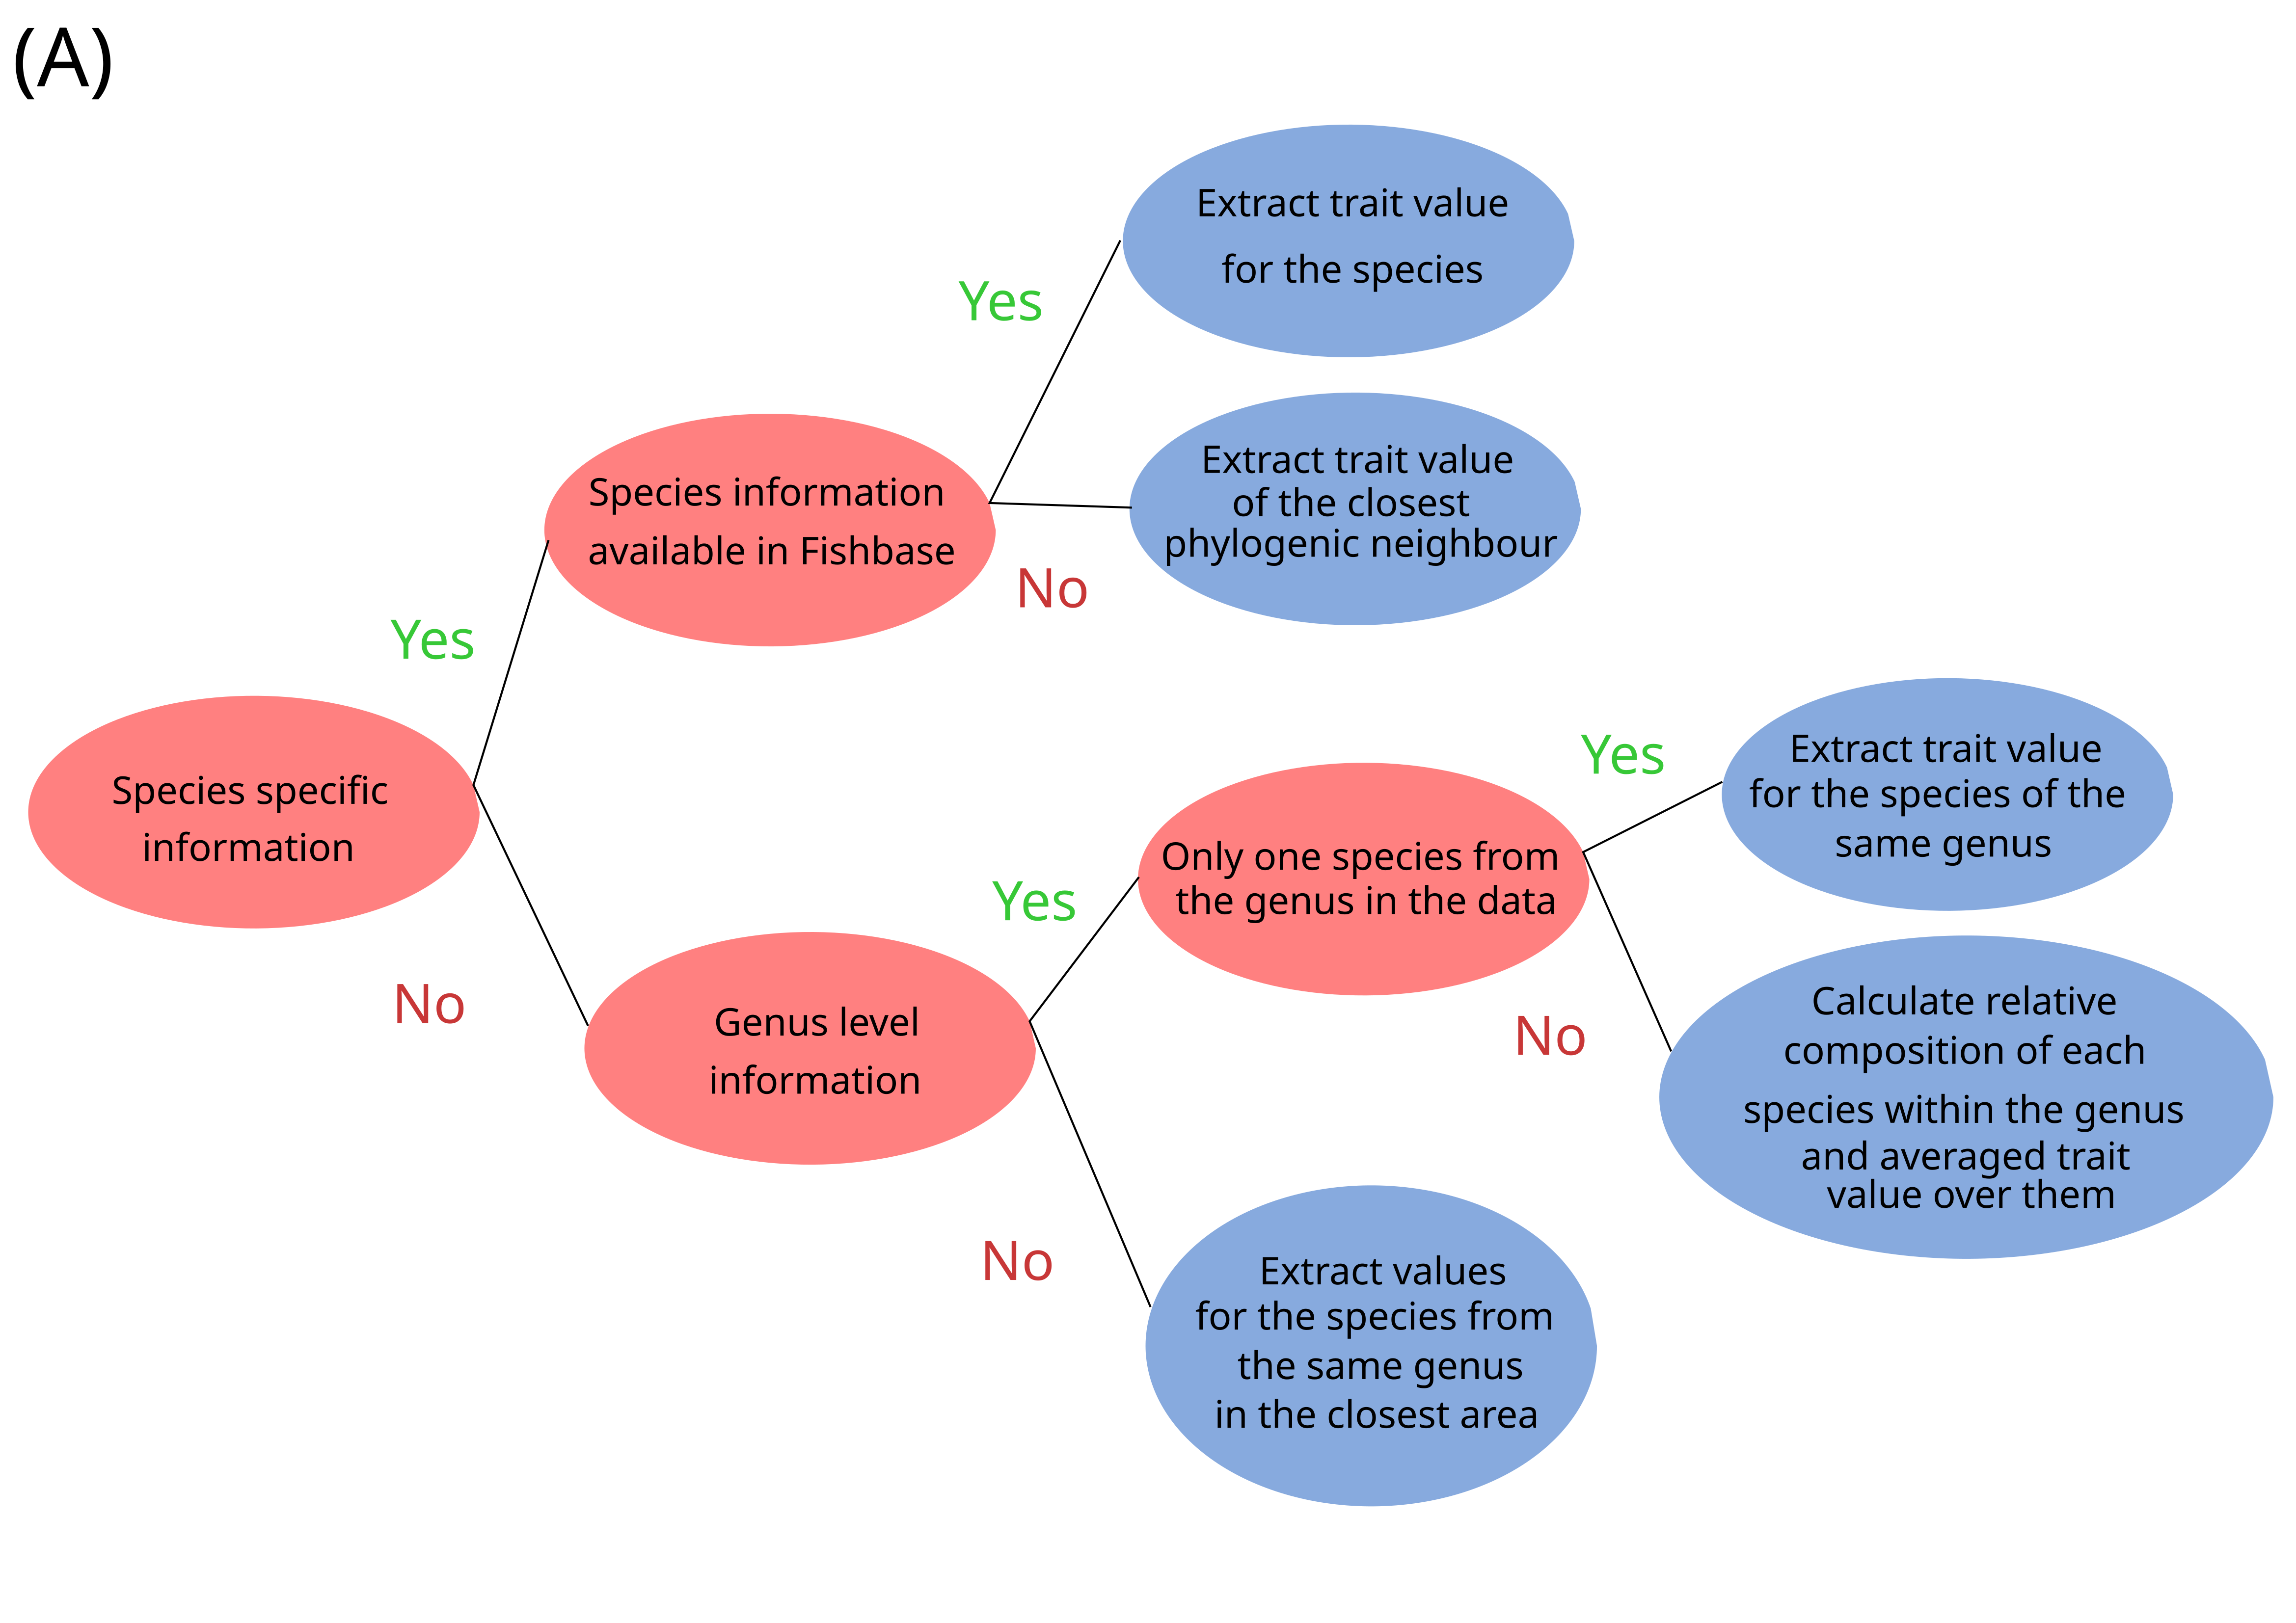
\includegraphics[width=1\linewidth]{Figures/decision_tree_fish} \caption{A caption}\label{fig:unnamed-chunk-2}
\end{figure}
\begin{figure}
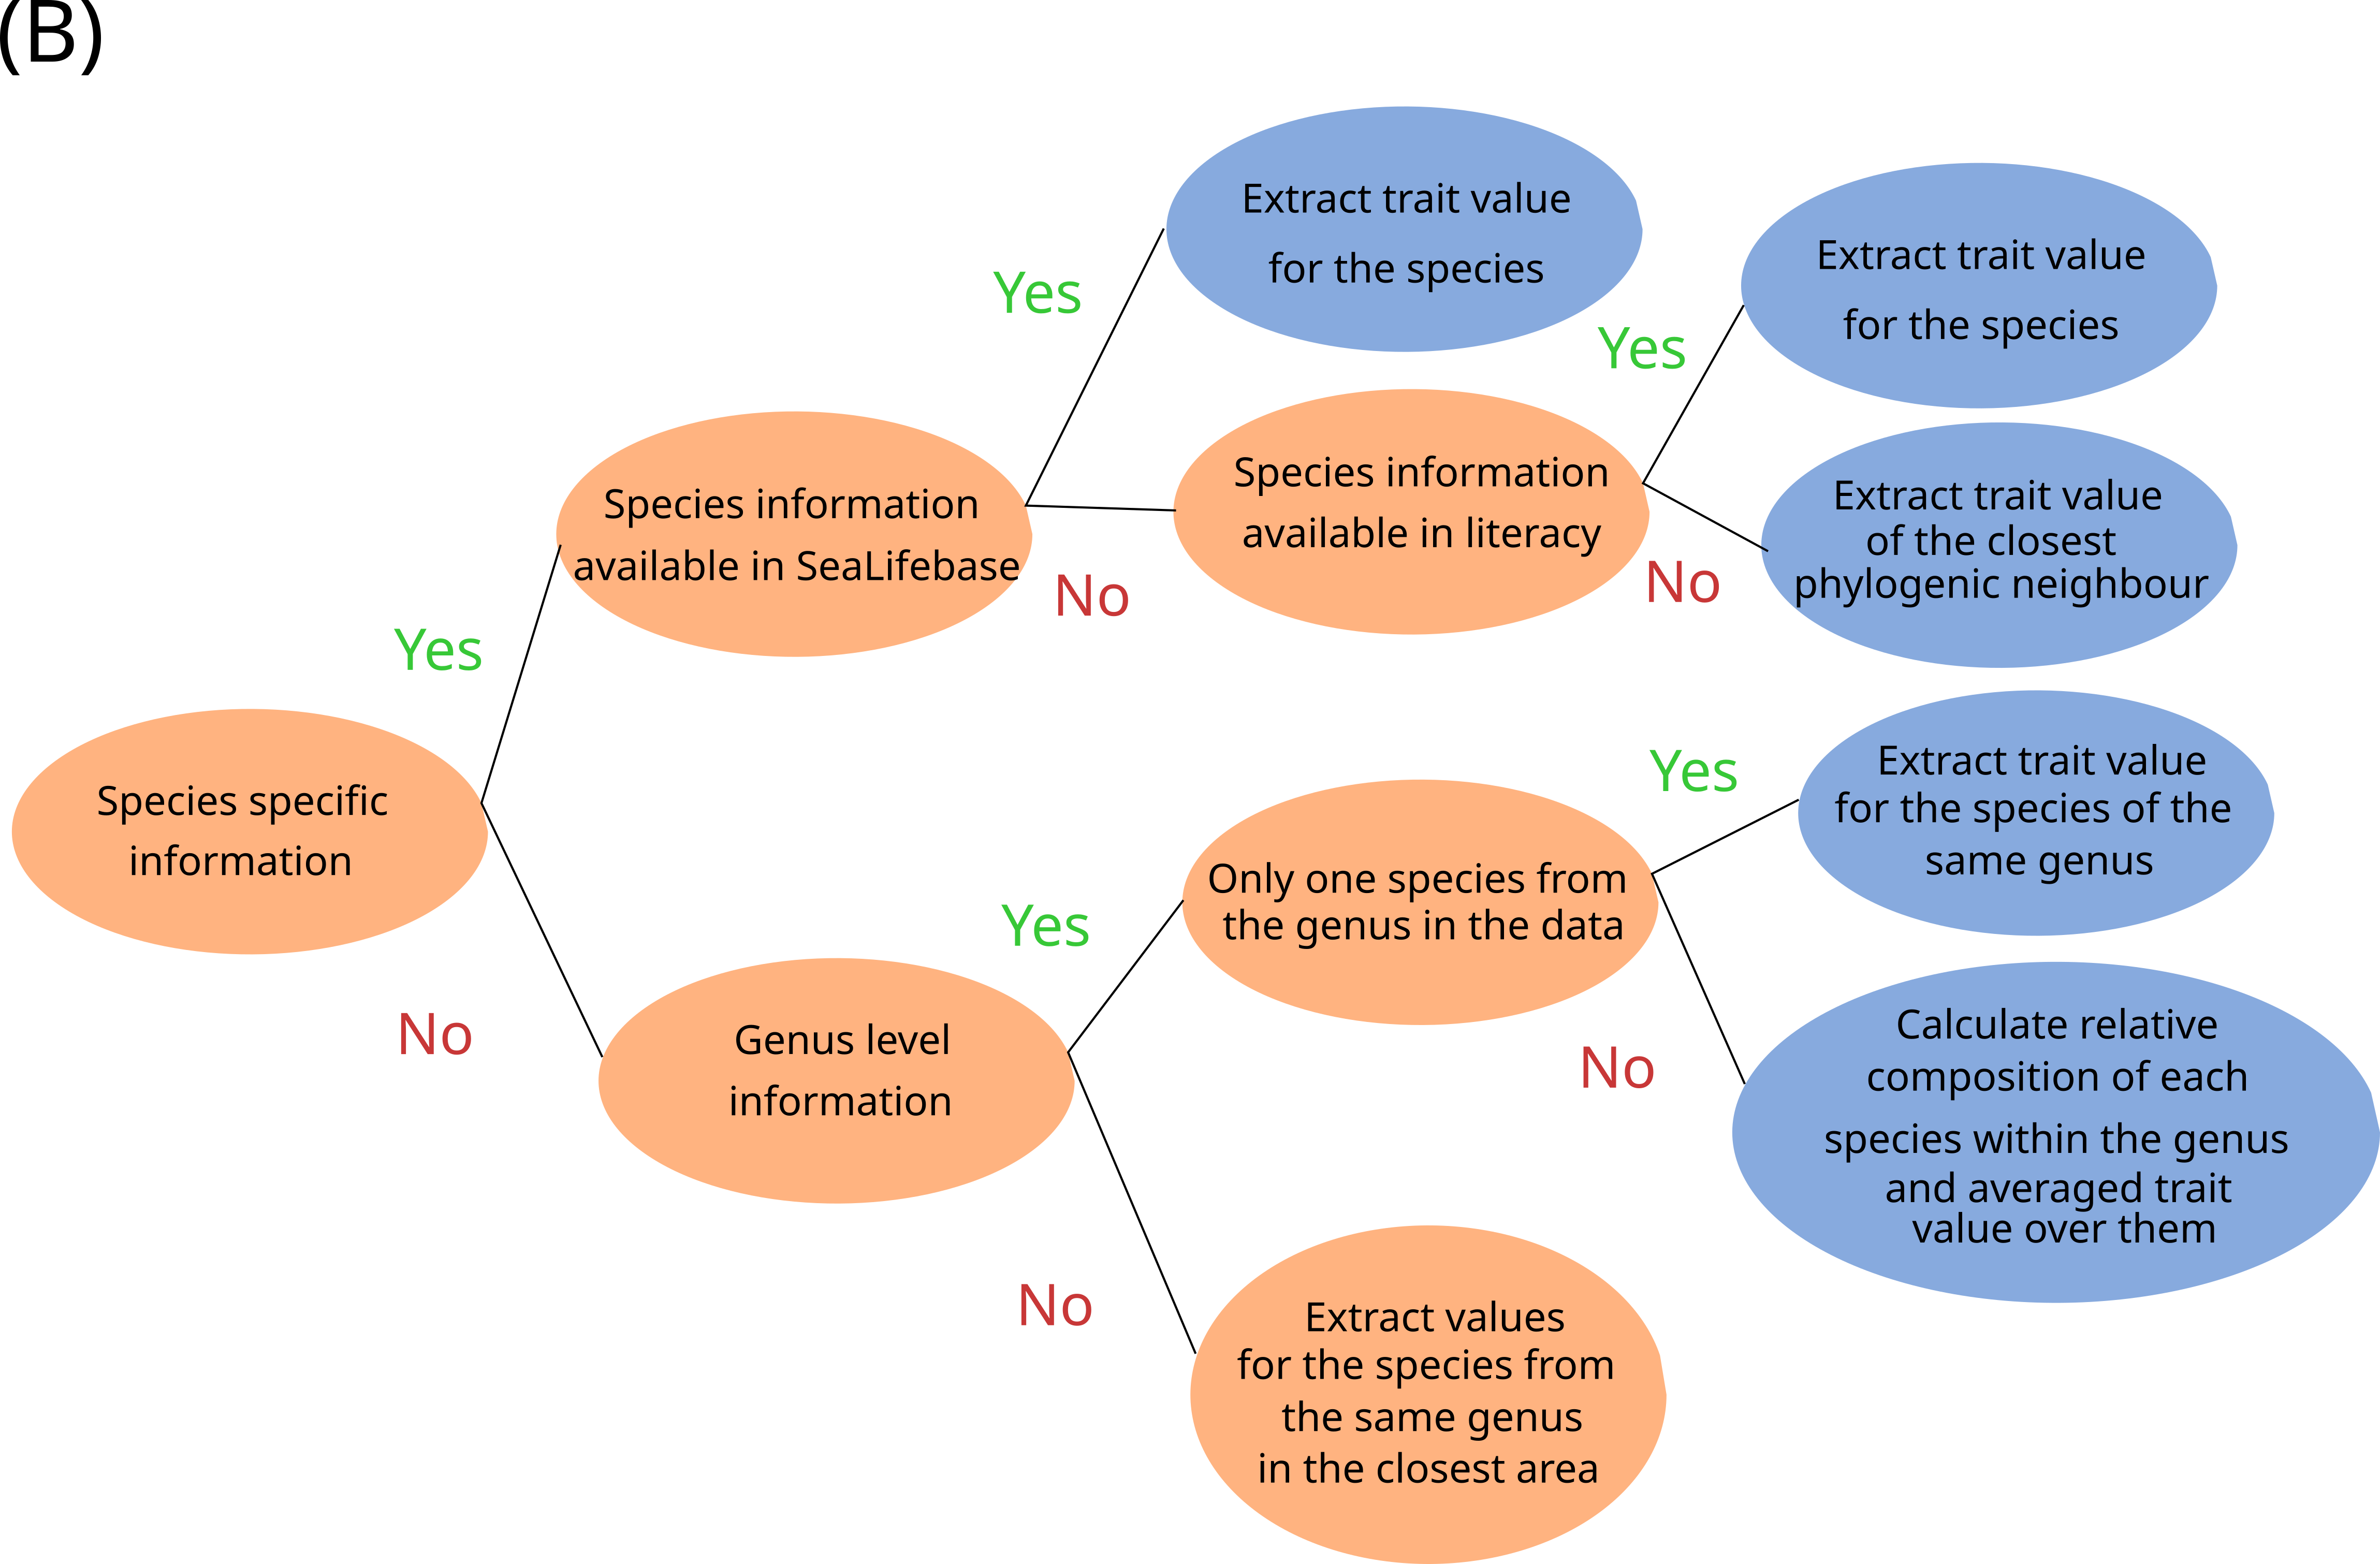
\includegraphics[width=1\linewidth]{Figures/decision_tree_cephalopods} \caption{A caption}\label{fig:unnamed-chunk-3}
\end{figure}

Open the correpsonding database

\begin{Shaded}
\begin{Highlighting}[]
\NormalTok{BDT\_FISH }\OtherTok{\textless{}{-}} \FunctionTok{read.csv}\NormalTok{(}\StringTok{"DATA/BDT\_FISH.csv"}\NormalTok{)}
\NormalTok{BDT\_CEPH}\OtherTok{\textless{}{-}} \FunctionTok{read.csv}\NormalTok{(}\StringTok{"DATA/BDT\_CEPHALO.csv"}\NormalTok{)}
\end{Highlighting}
\end{Shaded}

Correlation matrix for the selected traits

\begin{Shaded}
\begin{Highlighting}[]
\NormalTok{panel.cor.m }\OtherTok{\textless{}{-}} \ControlFlowTok{function}\NormalTok{(x, y, }\AttributeTok{digits=}\DecValTok{2}\NormalTok{)}
\NormalTok{\{}
\NormalTok{  usrold }\OtherTok{\textless{}{-}} \FunctionTok{par}\NormalTok{()}\SpecialCharTok{$}\NormalTok{usr; }\FunctionTok{on.exit}\NormalTok{(}\FunctionTok{par}\NormalTok{(}\StringTok{"usr"}\OtherTok{=}\NormalTok{usrold))}
  \FunctionTok{par}\NormalTok{(}\StringTok{"usr"} \OtherTok{=} \FunctionTok{c}\NormalTok{(}\DecValTok{0}\NormalTok{, }\DecValTok{1}\NormalTok{, }\DecValTok{0}\NormalTok{, }\DecValTok{1}\NormalTok{))}
\NormalTok{  r }\OtherTok{\textless{}{-}} \FunctionTok{cor}\NormalTok{(x, y,}\AttributeTok{method =} \StringTok{"spearman"}\NormalTok{, }\AttributeTok{use =} \StringTok{"complete.obs"}\NormalTok{)}
\NormalTok{  r2 }\OtherTok{\textless{}{-}} \FunctionTok{abs}\NormalTok{(}\FunctionTok{cor}\NormalTok{(x, y,}\AttributeTok{method =} \StringTok{"spearman"}\NormalTok{, }\AttributeTok{use =} \StringTok{"complete.obs"}\NormalTok{))}
\NormalTok{  txt }\OtherTok{\textless{}{-}} \FunctionTok{format}\NormalTok{(}\FunctionTok{c}\NormalTok{(r, }\FloatTok{0.123456789}\NormalTok{), }\AttributeTok{digits=}\NormalTok{digits)[}\DecValTok{1}\NormalTok{]}
\NormalTok{  cex }\OtherTok{\textless{}{-}} \FloatTok{0.8}\SpecialCharTok{/}\FunctionTok{strwidth}\NormalTok{(txt)}
  \FunctionTok{text}\NormalTok{(}\FloatTok{0.5}\NormalTok{, }\FloatTok{0.5}\NormalTok{, txt, }\AttributeTok{cex =}\NormalTok{ cex }\SpecialCharTok{*}\NormalTok{ r2)}
  
\NormalTok{\}}


\FunctionTok{pairs}\NormalTok{(BDT\_FISH[,}\DecValTok{2}\SpecialCharTok{:}\FunctionTok{ncol}\NormalTok{(BDT\_FISH)], }\AttributeTok{lower.panel=}\NormalTok{panel.smooth, }
      \AttributeTok{upper.panel=}\NormalTok{panel.cor.m)}
\end{Highlighting}
\end{Shaded}

\pandocbounded{\includegraphics[keepaspectratio]{Supporting_information_code_files/figure-latex/unnamed-chunk-5-1.pdf}}

\begin{Shaded}
\begin{Highlighting}[]
\FunctionTok{pairs}\NormalTok{(BDT\_CEPH[,}\DecValTok{2}\SpecialCharTok{:}\FunctionTok{ncol}\NormalTok{(BDT\_CEPH)], }\AttributeTok{lower.panel=}\NormalTok{panel.smooth, }
      \AttributeTok{upper.panel=}\NormalTok{panel.cor.m)}
\end{Highlighting}
\end{Shaded}

\pandocbounded{\includegraphics[keepaspectratio]{Supporting_information_code_files/figure-latex/unnamed-chunk-5-2.pdf}}

\section{2.2 Species abundance data}\label{species-abundance-data}

\begin{Shaded}
\begin{Highlighting}[]
\FunctionTok{load}\NormalTok{(}\StringTok{"DATA/abundance\_station\_species\_year\_fish.Rdata"}\NormalTok{)}
\NormalTok{fish\_abundance}\OtherTok{\textless{}{-}}\NormalTok{stock\_list\_abundance}
\FunctionTok{load}\NormalTok{(}\StringTok{"DATA/abundance\_station\_species\_year\_ceph.Rdata"}\NormalTok{)}
\NormalTok{ceph\_abundance}\OtherTok{\textless{}{-}}\NormalTok{stock\_list\_abundance}
\end{Highlighting}
\end{Shaded}

\section{2.3 Environmental data}\label{environmental-data}

With environmental variables followed by a x being the annual estimates
and environmental variables followed by a y being the `short
term'/`immediate snapshot' of the environmental variables at the time of
the sampling (november-december)

\begin{Shaded}
\begin{Highlighting}[]
 \FunctionTok{load}\NormalTok{(}\StringTok{"DATA/dataframe\_model\_2.Rdata"}\NormalTok{)}
\end{Highlighting}
\end{Shaded}

\section{2.4. Analysis}\label{analysis}

\subsection{2.4.1. Ecological traits Community Weighted Means
(CWMs)}\label{ecological-traits-community-weighted-means-cwms}

Calculate CWM for fish

\begin{Shaded}
\begin{Highlighting}[]
\CommentTok{\# keep only selected traits and homogenized species names}
\NormalTok{keepTraits }\OtherTok{\textless{}{-}} \FunctionTok{c}\NormalTok{(}\StringTok{"Mean\_temperature"}\NormalTok{,}\StringTok{"Max\_depth"}\NormalTok{,}\StringTok{"Range\_salinity"}\NormalTok{,}\StringTok{"Maximum\_body\_length"}\NormalTok{,}\StringTok{"Growth\_rate"}\NormalTok{,}\StringTok{"Fecundity"}\NormalTok{,}\StringTok{"Offspring\_size"}\NormalTok{,}\StringTok{"Age\_maturity"}\NormalTok{,}\StringTok{"Trophic\_level\_"}\NormalTok{)}
\NormalTok{BDT\_FISH}\SpecialCharTok{$}\NormalTok{SPECIES}\OtherTok{\textless{}{-}}\FunctionTok{gsub}\NormalTok{(}\StringTok{"\_"}\NormalTok{, }\StringTok{"."}\NormalTok{, BDT\_FISH}\SpecialCharTok{$}\NormalTok{SPECIES)}
\FunctionTok{rownames}\NormalTok{(BDT\_FISH)}\OtherTok{\textless{}{-}}\NormalTok{BDT\_FISH}\SpecialCharTok{$}\NormalTok{SPECIES}
\NormalTok{trait}\OtherTok{\textless{}{-}}\NormalTok{BDT\_FISH}
\NormalTok{trait }\OtherTok{\textless{}{-}}\NormalTok{ trait[,keepTraits]}
\NormalTok{abu}\OtherTok{\textless{}{-}}\FunctionTok{vector}\NormalTok{(}\StringTok{"list"}\NormalTok{, }\AttributeTok{length=}\DecValTok{24}\NormalTok{)}
\NormalTok{fishFD}\OtherTok{\textless{}{-}}\FunctionTok{vector}\NormalTok{(}\StringTok{"list"}\NormalTok{, }\AttributeTok{length=}\DecValTok{24}\NormalTok{)}

\CommentTok{\# create empty vector for all traits we are interested in }
\NormalTok{Mean\_temperature1}\OtherTok{\textless{}{-}}\NormalTok{Max\_Depth1}\OtherTok{\textless{}{-}}\NormalTok{Maximum\_body\_length1}\OtherTok{\textless{}{-}}\NormalTok{Fecundity1}\OtherTok{\textless{}{-}}\NormalTok{Offspring\_size1}\OtherTok{\textless{}{-}}\NormalTok{Trophic\_level\_1}\OtherTok{\textless{}{-}}\NormalTok{station1}\OtherTok{\textless{}{-}}\NormalTok{years1}\OtherTok{\textless{}{-}}\NormalTok{years2}\OtherTok{\textless{}{-}}\NormalTok{Range\_salinity1}\OtherTok{\textless{}{-}}\NormalTok{Growth\_rate1}\OtherTok{\textless{}{-}}\NormalTok{Age\_maturity1}\OtherTok{\textless{}{-}}\ConstantTok{NULL}
\NormalTok{Mean\_temperature}\OtherTok{\textless{}{-}}\NormalTok{Max\_Depth}\OtherTok{\textless{}{-}}\NormalTok{Maximum\_body\_length}\OtherTok{\textless{}{-}}\NormalTok{Fecundity}\OtherTok{\textless{}{-}}\NormalTok{Offspring\_size}\OtherTok{\textless{}{-}}\NormalTok{Trophic\_level\_}\OtherTok{\textless{}{-}}\NormalTok{stations}\OtherTok{\textless{}{-}}\NormalTok{Range\_salinity}\OtherTok{\textless{}{-}}\NormalTok{Growth\_rate}\OtherTok{\textless{}{-}}\NormalTok{Age\_maturity}\OtherTok{\textless{}{-}}\ConstantTok{NULL}

\CommentTok{\# loop over the years (i)}
\NormalTok{years}\OtherTok{\textless{}{-}}\FunctionTok{c}\NormalTok{(}\FunctionTok{seq}\NormalTok{(}\DecValTok{1997}\NormalTok{,}\DecValTok{2016}\NormalTok{),}\FunctionTok{seq}\NormalTok{(}\DecValTok{2018}\NormalTok{,}\DecValTok{2021}\NormalTok{))}
\ControlFlowTok{for}\NormalTok{ (i }\ControlFlowTok{in} \DecValTok{1}\SpecialCharTok{:}\DecValTok{24}\NormalTok{)\{}
  
\NormalTok{  abu1}\OtherTok{\textless{}{-}}\NormalTok{fish\_abundance[[i]]}
\NormalTok{  species}\OtherTok{\textless{}{-}}\FunctionTok{rownames}\NormalTok{(abu1)}
\NormalTok{  species}\OtherTok{\textless{}{-}} \FunctionTok{gsub}\NormalTok{(}\StringTok{" "}\NormalTok{, }\StringTok{"."}\NormalTok{, species)}
  \FunctionTok{rownames}\NormalTok{(abu1)}\OtherTok{\textless{}{-}}\NormalTok{species}
\NormalTok{  abu1}\OtherTok{\textless{}{-}}\NormalTok{abu1[, }\FunctionTok{colSums}\NormalTok{(abu1 }\SpecialCharTok{!=} \DecValTok{0}\NormalTok{) }\SpecialCharTok{\textgreater{}} \DecValTok{0}\NormalTok{]}
  
\NormalTok{  abu2}\OtherTok{\textless{}{-}}\FunctionTok{as.data.frame}\NormalTok{(}\FunctionTok{t}\NormalTok{(abu1))}
  
\NormalTok{  abu2}\OtherTok{\textless{}{-}}\NormalTok{abu2[, }\FunctionTok{colSums}\NormalTok{(abu2 }\SpecialCharTok{!=} \DecValTok{0}\NormalTok{) }\SpecialCharTok{\textgreater{}} \DecValTok{0}\NormalTok{]}
\NormalTok{  abu[[i]]}\OtherTok{\textless{}{-}}\NormalTok{abu2}
  
  
\NormalTok{  mtaxa }\OtherTok{\textless{}{-}} \FunctionTok{match}\NormalTok{(}\FunctionTok{colnames}\NormalTok{(abu[[i]]), }\FunctionTok{row.names}\NormalTok{(trait))}
  
  \CommentTok{\#check if there all species are matched: must be TRUE}
  \FunctionTok{all}\NormalTok{(}\SpecialCharTok{!}\FunctionTok{is.na}\NormalTok{(mtaxa))}
  
\NormalTok{  trait1 }\OtherTok{\textless{}{-}}\NormalTok{ trait[mtaxa,]}
  \FunctionTok{all}\NormalTok{(}\FunctionTok{colnames}\NormalTok{(abu[[i]])}\SpecialCharTok{==}\FunctionTok{row.names}\NormalTok{(trait1))}
  
\NormalTok{  fishFD[[i]]}\OtherTok{\textless{}{-}}\FunctionTok{dbFD}\NormalTok{(trait1, abu[[i]], }\AttributeTok{calc.FDiv =}\NormalTok{ F, }\AttributeTok{calc.FRic =}\NormalTok{ F) }
  

\NormalTok{  Mean\_temperature}\OtherTok{\textless{}{-}}\NormalTok{fishFD[[i]]}\SpecialCharTok{$}\NormalTok{CWM}\SpecialCharTok{$}\NormalTok{Mean\_temperature}
\NormalTok{  Max\_Depth}\OtherTok{\textless{}{-}}\NormalTok{fishFD[[i]]}\SpecialCharTok{$}\NormalTok{CWM}\SpecialCharTok{$}\NormalTok{Max\_depth}
\NormalTok{  Maximum\_body\_length}\OtherTok{\textless{}{-}}\NormalTok{fishFD[[i]]}\SpecialCharTok{$}\NormalTok{CWM}\SpecialCharTok{$}\NormalTok{Maximum\_body\_length}
\NormalTok{  Fecundity}\OtherTok{\textless{}{-}}\NormalTok{fishFD[[i]]}\SpecialCharTok{$}\NormalTok{CWM}\SpecialCharTok{$}\NormalTok{Fecundity}
\NormalTok{  Offspring\_size}\OtherTok{\textless{}{-}}\NormalTok{fishFD[[i]]}\SpecialCharTok{$}\NormalTok{CWM}\SpecialCharTok{$}\NormalTok{Offspring\_size}
\NormalTok{  Trophic\_level\_}\OtherTok{\textless{}{-}}\NormalTok{fishFD[[i]]}\SpecialCharTok{$}\NormalTok{CWM}\SpecialCharTok{$}\NormalTok{Trophic\_level\_}
\NormalTok{  Range\_salinity}\OtherTok{\textless{}{-}}\NormalTok{fishFD[[i]]}\SpecialCharTok{$}\NormalTok{CWM}\SpecialCharTok{$}\NormalTok{Range\_salinity}
\NormalTok{  Growth\_rate}\OtherTok{\textless{}{-}}\NormalTok{fishFD[[i]]}\SpecialCharTok{$}\NormalTok{CWM}\SpecialCharTok{$}\NormalTok{Growth\_rate}
\NormalTok{  Age\_maturity}\OtherTok{\textless{}{-}}\NormalTok{fishFD[[i]]}\SpecialCharTok{$}\NormalTok{CWM}\SpecialCharTok{$}\NormalTok{Age\_maturity}
  
\NormalTok{  stations}\OtherTok{\textless{}{-}}\FunctionTok{rownames}\NormalTok{(fishFD[[i]]}\SpecialCharTok{$}\NormalTok{CWM)}
\NormalTok{  years2}\OtherTok{\textless{}{-}}\FunctionTok{rep}\NormalTok{(years[[i]],}\FunctionTok{length}\NormalTok{(stations))}

\NormalTok{  Mean\_temperature1}\OtherTok{\textless{}{-}}\FunctionTok{c}\NormalTok{(Mean\_temperature,Mean\_temperature1)}
\NormalTok{  Max\_Depth1}\OtherTok{\textless{}{-}}\FunctionTok{c}\NormalTok{(Max\_Depth,Max\_Depth1)}
\NormalTok{  Maximum\_body\_length1}\OtherTok{\textless{}{-}}\FunctionTok{c}\NormalTok{(Maximum\_body\_length,Maximum\_body\_length1)}
\NormalTok{  Fecundity1}\OtherTok{\textless{}{-}}\FunctionTok{c}\NormalTok{(Fecundity,Fecundity1)}
\NormalTok{  Offspring\_size1}\OtherTok{\textless{}{-}}\FunctionTok{c}\NormalTok{(Offspring\_size,Offspring\_size1)}
\NormalTok{  Trophic\_level\_1}\OtherTok{\textless{}{-}}\FunctionTok{c}\NormalTok{(Trophic\_level\_,Trophic\_level\_1)}
\NormalTok{  Range\_salinity1}\OtherTok{\textless{}{-}}\FunctionTok{c}\NormalTok{(Range\_salinity,Range\_salinity1)}
\NormalTok{  Growth\_rate1}\OtherTok{\textless{}{-}}\FunctionTok{c}\NormalTok{(Growth\_rate,Growth\_rate1)}
\NormalTok{  Age\_maturity1}\OtherTok{\textless{}{-}}\FunctionTok{c}\NormalTok{(Age\_maturity,Age\_maturity1)}
\NormalTok{  station1}\OtherTok{\textless{}{-}}\FunctionTok{c}\NormalTok{(stations,station1)}
\NormalTok{  years1}\OtherTok{\textless{}{-}}\FunctionTok{c}\NormalTok{(years2,years1)}
  
\NormalTok{\}}
\end{Highlighting}
\end{Shaded}

\begin{verbatim}
## FEVe: Could not be calculated for communities with <3 functionally singular species. 
## FDis: Equals 0 in communities with only one functionally singular species.
\end{verbatim}

\begin{Shaded}
\begin{Highlighting}[]
\NormalTok{data\_for\_model}\OtherTok{\textless{}{-}}\FunctionTok{data.frame}\NormalTok{(}\AttributeTok{Mean\_temperature1=}\NormalTok{Mean\_temperature1,}
                           \AttributeTok{Max\_Depth1=}\NormalTok{Max\_Depth1,}
                           \AttributeTok{Maximum\_body\_length1=}\NormalTok{Maximum\_body\_length1,}
                           \AttributeTok{Fecundity1=}\NormalTok{Fecundity1,}
                           \AttributeTok{Offspring\_size1=}\NormalTok{Offspring\_size1,}
                           \AttributeTok{Trophic\_level\_1=}\NormalTok{Trophic\_level\_1,}
                           \AttributeTok{Range\_salinity1=}\NormalTok{Range\_salinity1,}
                           \AttributeTok{Growth\_rate1=}\NormalTok{Growth\_rate1,}
                           \AttributeTok{Age\_maturity1=}\NormalTok{Age\_maturity1,}
                           \AttributeTok{station=}\NormalTok{station1, }
                           \AttributeTok{years1=}\NormalTok{years1)}

\NormalTok{stations}\OtherTok{\textless{}{-}}\FunctionTok{unique}\NormalTok{(data\_for\_model}\SpecialCharTok{$}\NormalTok{station1)}
\NormalTok{stations\_2}\OtherTok{\textless{}{-}}\NormalTok{slope1}\OtherTok{\textless{}{-}}\NormalTok{pvalue1}\OtherTok{\textless{}{-}}\ConstantTok{NULL}

\FunctionTok{save}\NormalTok{(data\_for\_model, }\AttributeTok{file=}\StringTok{"data\_for\_model\_fish.Rdata"}\NormalTok{)}
\end{Highlighting}
\end{Shaded}

Calculate CWM for cephalopods

\begin{Shaded}
\begin{Highlighting}[]
\NormalTok{BDT\_CEPH}\SpecialCharTok{$}\NormalTok{SPECIES}\OtherTok{\textless{}{-}}\FunctionTok{gsub}\NormalTok{(}\StringTok{" "}\NormalTok{, }\StringTok{"."}\NormalTok{, BDT\_CEPH}\SpecialCharTok{$}\NormalTok{SPECIES)}
\FunctionTok{rownames}\NormalTok{(BDT\_CEPH)}\OtherTok{\textless{}{-}}\NormalTok{BDT\_CEPH}\SpecialCharTok{$}\NormalTok{SPECIES}
\NormalTok{trait}\OtherTok{\textless{}{-}}\NormalTok{BDT\_CEPH[,}\DecValTok{2}\SpecialCharTok{:}\FunctionTok{ncol}\NormalTok{(BDT\_CEPH)]}

\NormalTok{abu}\OtherTok{\textless{}{-}}\FunctionTok{vector}\NormalTok{(}\StringTok{"list"}\NormalTok{, }\AttributeTok{length=}\DecValTok{24}\NormalTok{)}
\NormalTok{cephFD}\OtherTok{\textless{}{-}}\FunctionTok{vector}\NormalTok{(}\StringTok{"list"}\NormalTok{, }\AttributeTok{length=}\DecValTok{24}\NormalTok{)}

\NormalTok{Mean\_temperature1}\OtherTok{\textless{}{-}}\NormalTok{Range\_temperature1}\OtherTok{\textless{}{-}}\NormalTok{Max\_Depth1}\OtherTok{\textless{}{-}}\NormalTok{Maximum\_body\_length1}\OtherTok{\textless{}{-}}\NormalTok{Fecundity1}\OtherTok{\textless{}{-}}\NormalTok{Trophic\_level\_1}\OtherTok{\textless{}{-}}\NormalTok{station1}\OtherTok{\textless{}{-}}\NormalTok{years1}\OtherTok{\textless{}{-}}\NormalTok{years2}\OtherTok{\textless{}{-}}\NormalTok{Length\_maturity1}\OtherTok{\textless{}{-}}\ConstantTok{NULL}
\NormalTok{Mean\_temperature}\OtherTok{\textless{}{-}}\NormalTok{Range\_temperature}\OtherTok{\textless{}{-}}\NormalTok{Max\_Depth}\OtherTok{\textless{}{-}}\NormalTok{Maximum\_body\_length}\OtherTok{\textless{}{-}}\NormalTok{Fecundity}\OtherTok{\textless{}{-}}\NormalTok{Trophic\_level\_}\OtherTok{\textless{}{-}}\NormalTok{stations}\OtherTok{\textless{}{-}}\NormalTok{Length\_maturity}\OtherTok{\textless{}{-}}\ConstantTok{NULL}


\NormalTok{years}\OtherTok{\textless{}{-}}\FunctionTok{c}\NormalTok{(}\FunctionTok{seq}\NormalTok{(}\DecValTok{1997}\NormalTok{,}\DecValTok{2016}\NormalTok{),}\FunctionTok{seq}\NormalTok{(}\DecValTok{2018}\NormalTok{,}\DecValTok{2021}\NormalTok{))}
\ControlFlowTok{for}\NormalTok{ (i }\ControlFlowTok{in} \DecValTok{1}\SpecialCharTok{:}\DecValTok{24}\NormalTok{)\{}
  
\NormalTok{  abu1}\OtherTok{\textless{}{-}}\NormalTok{ceph\_abundance[[i]]}
\NormalTok{  species}\OtherTok{\textless{}{-}}\FunctionTok{rownames}\NormalTok{(abu1)}
\NormalTok{  species}\OtherTok{\textless{}{-}} \FunctionTok{gsub}\NormalTok{(}\StringTok{" "}\NormalTok{, }\StringTok{"."}\NormalTok{, species)}
  \FunctionTok{rownames}\NormalTok{(abu1)}\OtherTok{\textless{}{-}}\NormalTok{species}
\NormalTok{  abu1}\OtherTok{\textless{}{-}}\NormalTok{abu1[, }\FunctionTok{colSums}\NormalTok{(abu1 }\SpecialCharTok{!=} \DecValTok{0}\NormalTok{) }\SpecialCharTok{\textgreater{}} \DecValTok{0}\NormalTok{]}
  
\NormalTok{  abu2}\OtherTok{\textless{}{-}}\FunctionTok{as.data.frame}\NormalTok{(}\FunctionTok{t}\NormalTok{(abu1))}
  
\NormalTok{  abu2}\OtherTok{\textless{}{-}}\NormalTok{abu2[, }\FunctionTok{colSums}\NormalTok{(abu2 }\SpecialCharTok{!=} \DecValTok{0}\NormalTok{) }\SpecialCharTok{\textgreater{}} \DecValTok{0}\NormalTok{]}
\NormalTok{  abu[[i]]}\OtherTok{\textless{}{-}}\NormalTok{abu2}
  
  
\NormalTok{  mtaxa }\OtherTok{\textless{}{-}} \FunctionTok{match}\NormalTok{(}\FunctionTok{colnames}\NormalTok{(abu[[i]]), }\FunctionTok{row.names}\NormalTok{(trait))}
  
  \CommentTok{\#check if there all species are matched: must be TRUE}
  \FunctionTok{all}\NormalTok{(}\SpecialCharTok{!}\FunctionTok{is.na}\NormalTok{(mtaxa))}
  
\NormalTok{  trait1 }\OtherTok{\textless{}{-}}\NormalTok{ trait[mtaxa,]}
  \FunctionTok{all}\NormalTok{(}\FunctionTok{colnames}\NormalTok{(abu[[i]])}\SpecialCharTok{==}\FunctionTok{row.names}\NormalTok{(trait1))}
  
\NormalTok{  cephFD[[i]]}\OtherTok{\textless{}{-}}\FunctionTok{dbFD}\NormalTok{(trait1, abu[[i]], }\AttributeTok{calc.FDiv =}\NormalTok{ F, }\AttributeTok{calc.FRic =}\NormalTok{ F)}
  
\NormalTok{  Mean\_temperature}\OtherTok{\textless{}{-}}\NormalTok{cephFD[[i]]}\SpecialCharTok{$}\NormalTok{CWM}\SpecialCharTok{$}\NormalTok{Mean\_temperature}
\NormalTok{  Range\_temperature}\OtherTok{\textless{}{-}}\NormalTok{cephFD[[i]]}\SpecialCharTok{$}\NormalTok{CWM}\SpecialCharTok{$}\NormalTok{Range\_temperature}
\NormalTok{  Max\_Depth}\OtherTok{\textless{}{-}}\NormalTok{cephFD[[i]]}\SpecialCharTok{$}\NormalTok{CWM}\SpecialCharTok{$}\NormalTok{Max\_depth}
\NormalTok{  Maximum\_body\_length}\OtherTok{\textless{}{-}}\NormalTok{cephFD[[i]]}\SpecialCharTok{$}\NormalTok{CWM}\SpecialCharTok{$}\NormalTok{Maximum\_length}
\NormalTok{  Fecundity}\OtherTok{\textless{}{-}}\NormalTok{cephFD[[i]]}\SpecialCharTok{$}\NormalTok{CWM}\SpecialCharTok{$}\NormalTok{Fecundity\_max}
\NormalTok{  Trophic\_level\_}\OtherTok{\textless{}{-}}\NormalTok{cephFD[[i]]}\SpecialCharTok{$}\NormalTok{CWM}\SpecialCharTok{$}\NormalTok{Trophic\_level}
\NormalTok{  Length\_maturity}\OtherTok{\textless{}{-}}\NormalTok{cephFD[[i]]}\SpecialCharTok{$}\NormalTok{CWM}\SpecialCharTok{$}\NormalTok{Length\_maturity}
\NormalTok{  stations}\OtherTok{\textless{}{-}}\FunctionTok{rownames}\NormalTok{(cephFD[[i]]}\SpecialCharTok{$}\NormalTok{CWM)}
\NormalTok{  years2}\OtherTok{\textless{}{-}}\FunctionTok{rep}\NormalTok{(years[[i]],}\FunctionTok{length}\NormalTok{(stations))}
  

\NormalTok{  Mean\_temperature1}\OtherTok{\textless{}{-}}\FunctionTok{c}\NormalTok{(Mean\_temperature,Mean\_temperature1)}
\NormalTok{  Range\_temperature1}\OtherTok{\textless{}{-}}\FunctionTok{c}\NormalTok{(Range\_temperature,Range\_temperature1)}
\NormalTok{  Max\_Depth1}\OtherTok{\textless{}{-}}\FunctionTok{c}\NormalTok{(Max\_Depth,Max\_Depth1)}
\NormalTok{  Maximum\_body\_length1}\OtherTok{\textless{}{-}}\FunctionTok{c}\NormalTok{(Maximum\_body\_length,Maximum\_body\_length1)}
\NormalTok{  Fecundity1}\OtherTok{\textless{}{-}}\FunctionTok{c}\NormalTok{(Fecundity,Fecundity1)}
\NormalTok{  Trophic\_level\_1}\OtherTok{\textless{}{-}}\FunctionTok{c}\NormalTok{(Trophic\_level\_,Trophic\_level\_1)}
\NormalTok{  Length\_maturity1}\OtherTok{\textless{}{-}}\FunctionTok{c}\NormalTok{(Length\_maturity,Length\_maturity1)}
\NormalTok{  station1}\OtherTok{\textless{}{-}}\FunctionTok{c}\NormalTok{(stations,station1)}
\NormalTok{  years1}\OtherTok{\textless{}{-}}\FunctionTok{c}\NormalTok{(years2,years1)}
  
\NormalTok{\}}


\NormalTok{data\_for\_model}\OtherTok{\textless{}{-}}\FunctionTok{data.frame}\NormalTok{(}\AttributeTok{Mean\_temperature1=}\NormalTok{Mean\_temperature1,}
                           \AttributeTok{Range\_temperature1=}\NormalTok{Range\_temperature1,}
                           \AttributeTok{Max\_Depth1=}\NormalTok{Max\_Depth1,}
                           \AttributeTok{Maximum\_body\_length1=}\NormalTok{Maximum\_body\_length1,}
                           \AttributeTok{Fecundity1=}\NormalTok{Fecundity1,}
                           \AttributeTok{Trophic\_level\_1=}\NormalTok{Trophic\_level\_1,}
                           \AttributeTok{Length\_maturity1=}\NormalTok{Length\_maturity1,}
                           \AttributeTok{station=}\NormalTok{station1, }
                           \AttributeTok{years1=}\NormalTok{years1)}

\NormalTok{stations}\OtherTok{\textless{}{-}}\FunctionTok{unique}\NormalTok{(data\_for\_model}\SpecialCharTok{$}\NormalTok{station1)}
\NormalTok{stations\_2}\OtherTok{\textless{}{-}}\NormalTok{slope1}\OtherTok{\textless{}{-}}\NormalTok{pvalue1}\OtherTok{\textless{}{-}}\ConstantTok{NULL}


\FunctionTok{save}\NormalTok{(data\_for\_model, }\AttributeTok{file=}\StringTok{"data\_for\_model\_cephalo.Rdata"}\NormalTok{)}
\end{Highlighting}
\end{Shaded}

\subsection{2.4.2 Correlative relation between environmental predictors
and
CWMs}\label{correlative-relation-between-environmental-predictors-and-cwms}

\subsection{2.4.3. Clustering CWM linear trends to determine spatial
patterns associated to temporal changes in community
traits}\label{clustering-cwm-linear-trends-to-determine-spatial-patterns-associated-to-temporal-changes-in-community-traits}

\end{document}
